%%%%%%%%%%%%%%%%%%%%%%%%%%%%%%%%%%%%%%%%%%%%%%%%%%%%%%%%%%%%%%%%%%%%%%%%%%%%%%%%%%%
%% This project aims to create the UNAL template for presentation.               %%
%% author:Félix Julián Gutiérrez                                                 %%
%% contacts:                                                                     %%
%%    e-mail: fjgutierrezb@unal.edu.co                                           %%
%%   www.unal.edu.co                                                             %%
%%%%%%%%%%%%%%%%%%%%%%%%%%%%%%%%%%%%%%%%%%%%%%%%%%%%%%%%%%%%%%%%%%%%%%%%%%%%%%%%%%%
\documentclass{libs/ufc_format}
% Inserting the preamble file with the packages
%%%%%%%%%%%%%%%%%%%%%%%%%%%%%%%%%%%%%%%%%%%%%%%%%%%%%%%%%%%%%%%%%%%%%
%% This file contains the packages that can be used in the beamer. %%
%%%%%%%%%%%%%%%%%%%%%%%%%%%%%%%%%%%%%%%%%%%%%%%%%%%%%%%%%%%%%%%%%%%%%
% Package to fonts family
\usepackage[T1]{fontenc}
% Package to accentuation
\usepackage[utf8]{inputenc}
% Package to Spanish language
\usepackage[spanish]{babel}
% Package to Figures
\usepackage{graphicx}
% Package to the colors
\usepackage{color}
% Package to the colors
\usepackage{xcolor}
% Packages to math symbols and expressions
\usepackage{amsfonts, amssymb, amsmath}
% Package to multiple lines and columns in table
\usepackage{multirow, array} 
% Package to create pseudo-code
% For more detail of this package: http://linorg.usp.br/CTAN/macros/latex/contrib/algorithm2e/doc/algorithm2e.pdf
\usepackage{algorithm2e}
% Package to insert code
\usepackage{listings} 
\usepackage{keyval}
% Package to justify text
\usepackage[document]{ragged2e}
% Package to manage the bibliography
\usepackage[backend=biber, style=numeric, sorting=none]{biblatex}
% Package to facilities quotations
\usepackage{csquotes}
% Package to use multicols
\usepackage{multicol}

% SVG (CUSTOM)
\usepackage{svg}
% Inserting the references file
\bibliography{references.bib}

% Title
\title[Sistemas Operativos]{\huge\textbf{}}
% Subtitle
\subtitle{\textbf{El Sistema Operativo XV6 - Capitulo 1}}
% Author of the presentation
\author{Carlos Santiago Sandoval Casallas}
% Institute's Name
\institute[UNAL]{
  % email for contact
  \normalsize{\email{csandovalc@unal.edu.co}}
  \newline
  % Department Name
  \department{Departamento de Ingeniería de Sistemas e Industrial}
  \newline
  % university name
  \ufc
}
% date of the presentation
\date{\today}

%%%%%%%%%%%%%%%%%%%%%%%%%%%%%%%%%%%%%%%%%%%%%%%%%%%%%%%%%%%%%%%%%%%%%%%%%%%%%%%%%%
%% Start Document of the Presentation                                           %%
%%%%%%%%%%%%%%%%%%%%%%%%%%%%%%%%%%%%%%%%%%%%%%%%%%%%%%%%%%%%%%%%%%%%%%%%%%%%%%%%%%
\begin{document}
% insert the code style
%%%%%%%%%%%%%%%%%%%%%%%%%%%%%%%%%%%%%%%%%%%%%%%%%%%%%%%%%%%%%%%%%%%%%%%%%%%%%%%%%%%
%% This file contains the style of the codes show in slides.                     %%
%% The package used is listings, but it possible to used others.                 %%
%%%%%%%%%%%%%%%%%%%%%%%%%%%%%%%%%%%%%%%%%%%%%%%%%%%%%%%%%%%%%%%%%%%%%%%%%%%%%%%%%%%

% color used in the code style
\definecolor{codegreen}{rgb}{0,0.6,0}
\definecolor{codegray}{rgb}{0.5,0.5,0.5}
\definecolor{codepurple}{rgb}{0.58,0,0.82}
\definecolor{codebackground}{rgb}{0.95,0.95,0.92}

% style of the code!
\lstdefinestyle{codestyle}{
    backgroundcolor=\color{codebackground},   
    commentstyle=\color{codegreen},
    keywordstyle=\color{magenta},
    numberstyle=\tiny\color{codegray},
    stringstyle=\color{codepurple},
    basicstyle=\ttfamily\footnotesize,
    frame=single,
    breakatwhitespace=false,         
    breaklines=true,                 
    captionpos=b,                    
    keepspaces=true,                 
    numbers=left,                    
    numbersep=5pt,                  
    showspaces=false,                
    showstringspaces=false,
    showtabs=false,                  
    tabsize=2,
    title=\lstname 
}

\lstset{style=codestyle}


%% ---------------------------------------------------------------------------
% First frame (with tile, subtitle, ...)
\begin{frame}{}
  \maketitle
\end{frame}

%% ---------------------------------------------------------------------------
% Second frame
\begin{frame}{Agenda}
  % \begin{multicols}{2}
  \tableofcontents
  % \end{multicols}
\end{frame}
%% ---------------------------------------------------------------------------
\section{Interfaces del SO}
\begin{frame}{¿Cuál es la finalidad de un sistema operativo?}
  Los objetivos principales de los sistemas operativos son:
  \begin{itemize}
    \item Gestionar los recursos físicos y simplificar su administración para otros programas
      \newline\example{Un procesador de textos no necesita preocuparse por el tipo de disco empleado}
    \item Soportar la ejecución de múltiples programas en paralelo
      \newline\example{Un editor de texto y un navegador ejecutándose al mismo tiempo}
    \item Proporcionar métodos controlados para la interacción entre programas
      \newline\example{Tuberías, paso de mensajes}
  \end{itemize}
\end{frame}
%% ---------------------------------------------------------------------------
\begin{frame}{Diseño de interfaces}
  El concepto de interfaz es empleado para hacer referencia a una conexión funcional entre sistemas, programas, dispositivos, etc. \cite{wiki:Interfaz}\newline

  \vspace{0.4cm}

  El diseño de estas interfaces se basa en crear pocos mecanismos que sean combinables entre sí para cumplir necesidades más complejas, proporcionando generalidad y facilitando la implementación.

  \vspace{0.4cm}

  En este caso se trabajará sobre XV6, un sistema operativo educativo desarrollado y mantenido por el MIT. Este sistema proporciona las interfaces básicas basadas en el sistema operativo Unix V6 \cite{xv6_book}, además de imitar su diseño.
\end{frame}
%% ---------------------------------------------------------------------------
\begin{frame}{}
  \begin{figure}
    \centering
    \caption{Estructura de sistema operativo con su espacio de usuario}
    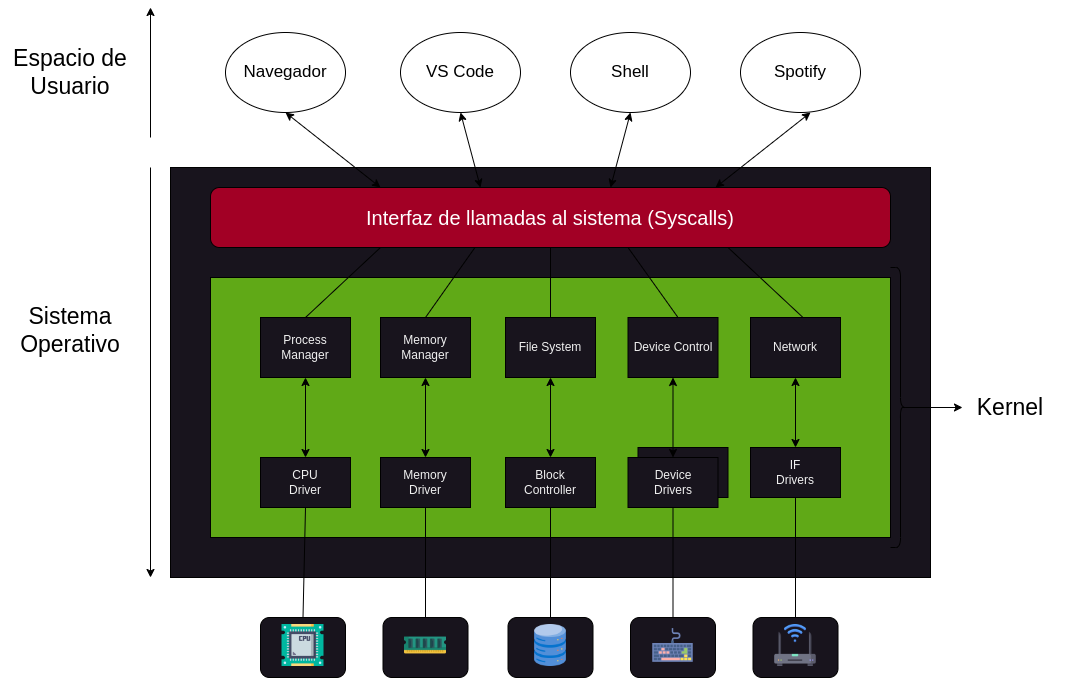
\includegraphics[scale=0.25]{libs/img/Estructura_kernel.png}
    \source{Elaboración propia. Iconos obtenidos del sitio Flaticon.com}
    \label{fig:Estructura Kernel}
  \end{figure}
\end{frame}
%% ---------------------------------------------------------------------------
\section{Procesos y memoria}
\begin{frame}{Procesos y el kernel}
  Cada programa en ejecución tiene el nombre de proceso, el kernel o núcleo, es un proceso especial que brinda servicios a los programas en ejecución, una computadora típicamente tiene muchos proceso pero solo un kernel.

  \vspace{0.4cm}

  Cuando un proceso necesita emplear uno de los servicios proporcionados por el kernel, invoca una llamada al sistema o \textit{syscall}, la llamada ingresa al espacio de kernel, el kernel realiza el servicio solicitado y regresa al programa desde donde ha sido invocado. \newline

  \vspace{0.2cm}

  \example{Un proceso alterna entre ejecutarse en el espacio de usuario y el espacio del kernel}
\end{frame}
%% ---------------------------------------------------------------------------
\begin{frame}{}
  El kernel emplea algunos mecanismos de protección proporcionados por el hardware, para garantizar que un proceso que se ejecuta en el espacio de usuario pueda acceder solo a su propia memoria. Mientras que el kernel ejecuta instrucciones con estos privilegios sobre el hardware para implementar dichas protecciones.

  \vspace{0.3cm}

  Cuando un programa desde el espacio de usuario invoca una syscall, el hardware aumenta el nivel de privilegio para ejecutar la función \emph{ya preestablecida en el kernel}.

  \vspace{0.2cm}

  \begin{block}{User mode, supervisor mode, and system calls}
    Esto se explorará con mayor profundidad en el capítulo 2.2
  \end{block}
\end{frame}
%% ---------------------------------------------------------------------------
\begin{frame}
  \begin{figure}
    \centering
    \caption{Llamadas al sistema disponibles en XV6. Si no se indica lo contrario retornan -1 si hay error y 0 en otro caso.}
    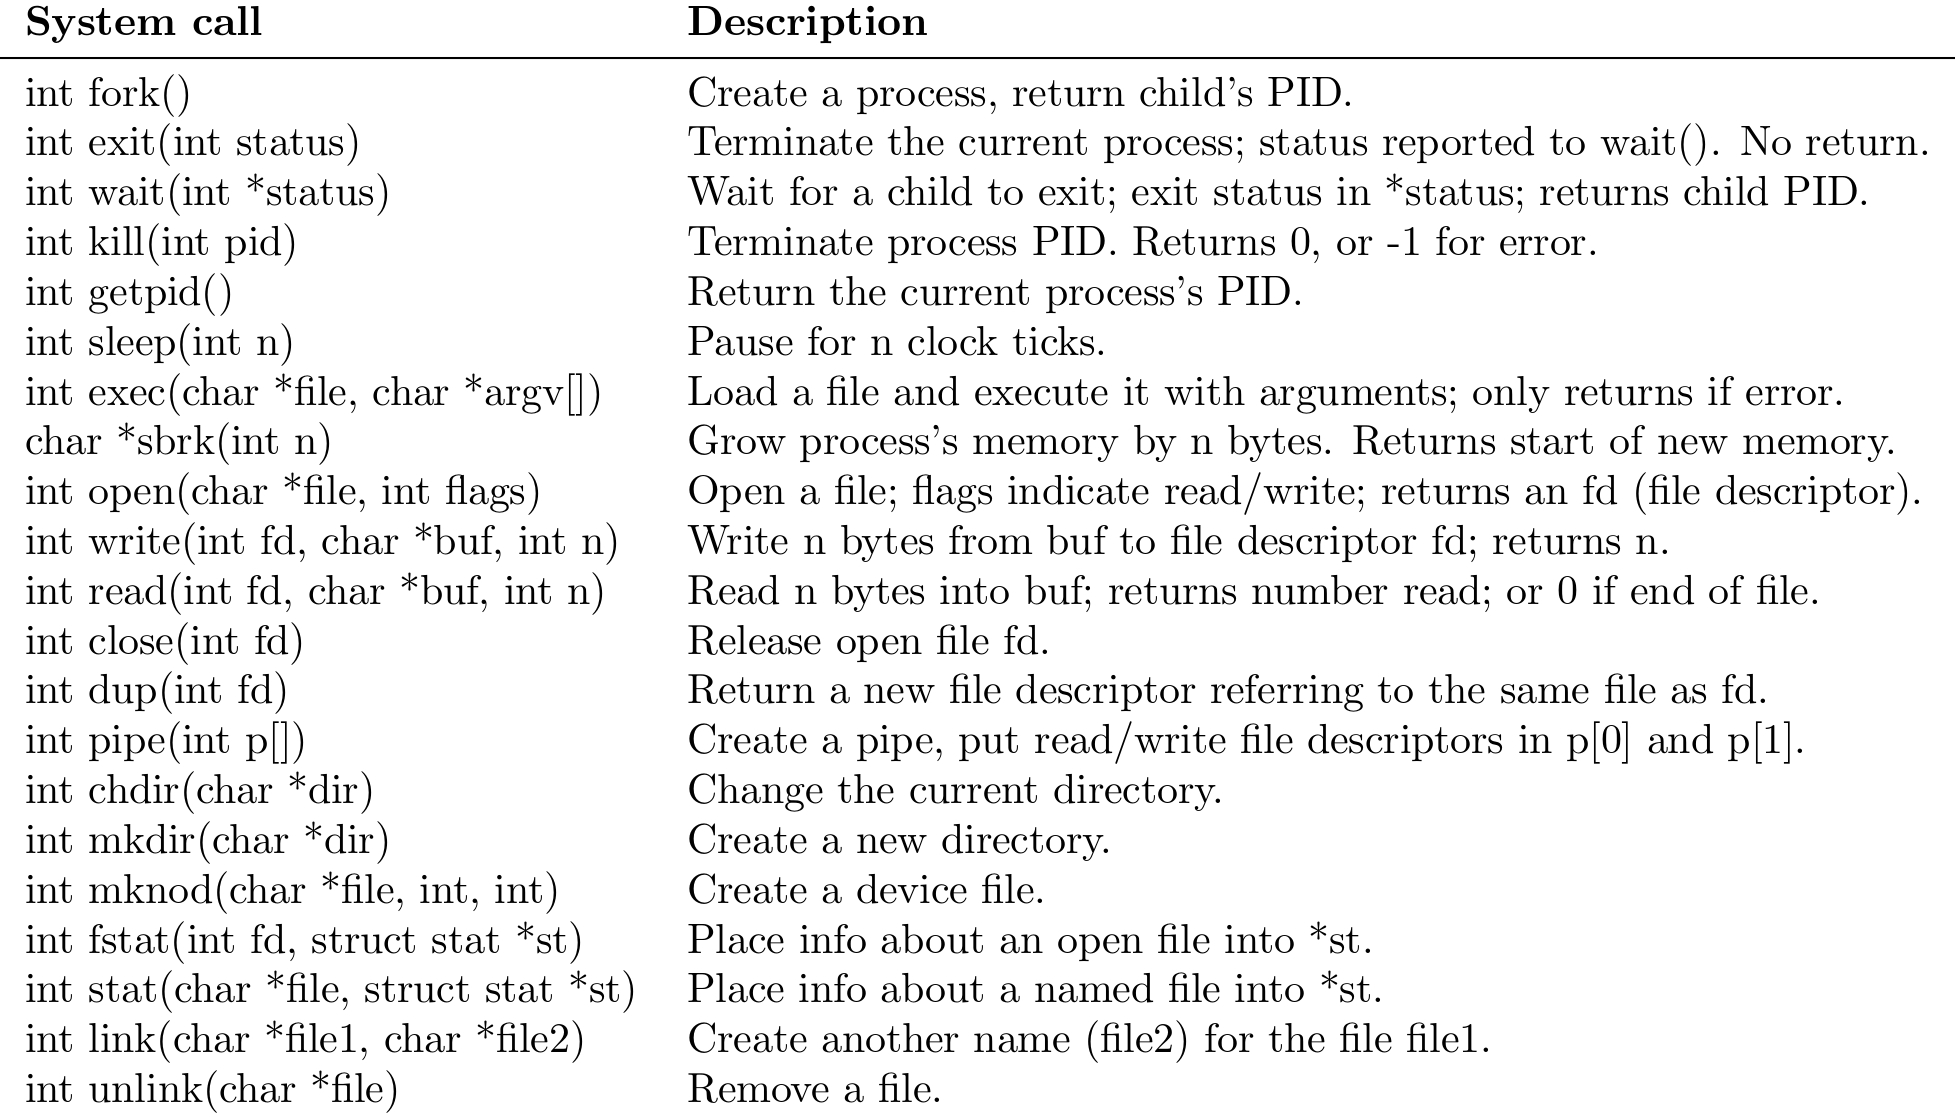
\includegraphics[scale=0.6]{libs/img/syscalls.jpg}
    \source{Tomado de xv6: a simple, Unix-like teaching operating system \cite{xv6_book}}
    \label{fig:Syscalls}
  \end{figure}
\end{frame}
%% ---------------------------------------------------------------------------
\begin{frame}{Aplicación de las llamadas al sistema}
  \lstinputlisting[language=C]{code/syscall_example.c}
\end{frame}
%% ---------------------------------------------------------------------------
\begin{frame}{}
  Las llamadas al sistema empleadas son:
  \begin{itemize}
    \item \textbf{fork:} Crea un nuevo proceso, este es un duplicado del proceso que emplea la llamada del sistema, el nuevo proceso es referido como \textit{proceso hijo}. El proceso que empleo la syscall es referido como \textit{proceso padre}.
    \item \textbf{wait:} Retorna el PID del proceso hijo que ha sufrido de un cambio de estado, estos pueden ser que el hijo: ha salido (exit), ha sido eliminado (killed), ha sido detenido o reanudado por una señal, este copia el estado de salida del proceso hijo.
    \item \textbf{exit:} Terminar la ejecución del proceso que lo llama, liberando recursos como memoria y archivos abiertos. Este toma un argumento de tipo entero, este es el \textit{status}, al momento de invocar la syscall, se retorna el byte menos significativo a su proceso padre. \newline
  \end{itemize}
  \emph{Toda la información puede ser encontrada en las man pages de Linux}
\end{frame}
%% ---------------------------------------------------------------------------
\begin{frame}{Fork}
  Fork crea una réplica del proceso, donde tanto el proceso padre como el hijo poseen el mismo contenido en memoria, esta se encuentra en lugares diferentes de la memoria y emplean registros separados, por lo que cambiar una variable en un proceso, no afecta al otro.
\end{frame}
%% ---------------------------------------------------------------------------
\begin{frame}{Shell}
  El Shell es un programa ordinario que lee los comandos del usuario y los ejecuta. Este se ejecuta en el espacio de usuario, su funcionamiento es apoyado principalmente por las syscall de \textit{fork} y \textit{exec}.
  \begin{itemize}
    \item \textbf{exec:} Reemplaza la memoria del proceso que llama con una nueva imagen de memoria cargada desde un archivo almacenado en el sistema de archivos. El archivo debe tener un formato particular, XV6 emplea el formato ELF.
      \begin{block}{Formato ELF}
        Este se verá con mayor detalle en el capítulo 3.8
      \end{block}
  \end{itemize}
\end{frame}
%% ---------------------------------------------------------------------------
\begin{frame}{Ejemplo de Exec}
  \lstinputlisting[language=C]{code/exec_example.c}
\end{frame}
%% ---------------------------------------------------------------------------
\begin{frame}
  En el código anterior, se reemplaza el programa con una instancia del binario en \textit{/bin/echo} que se ejecuta con la lista de argumentos \textit{argv}.

  \vspace{0.3cm}

  El bucle principal de la Shell \href{https://github.com/CarlosSandoval-03/xv6-riscv/blob/riscv/user/sh.c\#L146}{\textbf{\textit{(user/sh.c:146)}}} \cite{xv6} lee el input del usuario con el método \textit{getcmd}. Se emplea un fork, el padre espera, mientras que el proceso hijo ejecuta el comando. Si exec tiene éxito, el proceso hijo ejecutará las instrucciones del binario ejecutado, cuando estos finalicen, el padre finaliza la espera y continua con la ejecución.

  \vspace{0.3cm}

  El programa del Shell aprovecha la separación en su implementación de la redirección de E/S. Esto para evitar el desperdicio de crear un proceso duplicado y luego reemplazarlo de inmediato.
\end{frame}
%% ---------------------------------------------------------------------------
\begin{frame}{Asignación de memoria del espacio de usuario}
  XV6 asigna la mayor parte de la memoria del espacio de usuario implícitamente; fork asigna la memoria requerida para la copia del proceso, mientras exec asigna suficiente memoria para contener el ejecutable. En caso de requerir más memoria en tiempo de ejecución, se puede emplear \textit{sbrk(n)} para aumentar la memoria en \textit{n} bytes.

  \begin{block}{sbrk}
    Este se verá con mayor detalle en el capítulo 3.7
  \end{block}
\end{frame}

%% ---------------------------------------------------------------------------
\section{E/S y descriptores de archivo}
\begin{frame}{Descriptor de Archivo}
  Un descriptor es un entero que representa un objeto administrado por el kernel, este puede ser empleado para administrar: un archivo, directorio o dispositivo. La interfaz del descriptor de archivos, el objeto para que sea manipulado como un flujo de entrada o salida de bytes.

  \vspace{0.4cm}

  El kernel de XV6 asigna el valor del descriptor a un índice de una tabla \textit{por proceso}, permitiendo que cada proceso tenga un espacio privado de descriptores que inician en cero.

  \vspace{0.4cm}

  Existe una convención respecto a ciertos descriptores, estos son:
  \begin{itemize}
    \item \textbf{0:} Entrada estándar
    \item \textbf{1:} Salida estándar
    \item \textbf{2:} Error estándar
  \end{itemize}
\end{frame}
%% ---------------------------------------------------------------------------
\begin{frame}{Aplicación de los descriptores}
  El Shell, se encarga de emplear los descriptores estándar, de esta manera puede usarlos en la canalización (uso de tuberías) o redirección de E/S. Para esto el Shell verifica tener estos descriptores abiertos
  \href{https://github.com/CarlosSandoval-03/xv6-riscv/blob/riscv/user/sh.c\#L152}{\textbf{\textit{(user/sh:152)}}}. \cite{xv6}

  \vspace{0.2cm}

  Como emplear estos descriptores mediante las interfaces del sistema:
  \begin{itemize}
    \item \textit{read(fd, buff, n):} \textit{\example{fd}} es el descriptor del objeto sobre el cual se quiere leer, \textit{\example{buff}} la referencia en donde se almacenaran los \textit{\example{n}} bytes leídos.
    \item \textit{write(fd, buff, n):} \textit{\example{fd}} es el descriptor del objeto sobre el cual se quiere escribir, \textit{\example{buff}} la referencia de donde salen los \textit{\example{n}} bytes a escribir.
  \end{itemize}
  \emph{Cada archivo referenciado por un descriptor, tiene un desplazamiento asociado}
\end{frame}
%% ---------------------------------------------------------------------------
\begin{frame}{Ejemplo sobre el uso de descriptores estándar}
  Una implementación simple que sobre la lectura y escritura estándar:
  \lstinputlisting[language=C, basicstyle=\tiny]{code/descriptors_example.c}
\end{frame}
%% ---------------------------------------------------------------------------
\begin{frame}{Close}
  La llamada al sistema \textit{close}, libera un descriptor de archivo, lo que permite su reutilización para otra llamada al sistema, una canalización (pipe) o duplicación (dup). Un descriptor de archivo recién asignado siempre será, el número más bajo disponible \emph{(no utilizado)} en el proceso actual.

  \vspace{0.3cm}

  Los descriptores tienen ciertas interacciones con \textit{fork} y \textit{exec}. \textit{Fork} copiará la tabla de descriptores, por lo tanto, ambos procesos tendrán acceso a los mismos archivos. \textit{Exec} por su parte, reemplaza la memoria del proceso con la nueva imagen solicitada, \emph{pero conservará la tabla de archivos}.

  \vspace{0.2cm}

  \example{Esto permite que el Shell implemente la redirección de E/S usando fork y posteriormente empleando exec para ejecutar el nuevo programa.}
\end{frame}
%% ---------------------------------------------------------------------------
\begin{frame}{Redirección mediante syscalls}
  El siguiente programa ejemplifica el comando \textit{cat < input.txt}
  \lstinputlisting[language=C, basicstyle=\tiny]{code/cat_example.c}
\end{frame}
%% ---------------------------------------------------------------------------
\begin{frame}{Explicación}
  En el código anterior, el proceso hijo cierra el descriptor 0, de esta manera garantizamos que al momento de abrir el archivo \textit{input.txt} este se le asigne el descriptor más pequeño posible, posteriormente \textit{cat} se ejecuta, con el descriptor 0, pero en este caso hará referencia al archivo \textit{input.txt} y no a la entrada estándar.
  \emph{Este proceso no afectará los descriptores del proceso padre}

  \vspace{0.4cm}

  Esto se puede ver en profundidad en \href{https://github.com/CarlosSandoval-03/xv6-riscv/blob/riscv/user/sh.c\#L83}{\textbf{\textit{(user/sh.c:83)}}} \cite{xv6}, al momento de ejecutarse este código, ya se ha bifurcado el Shell y \textit{runcmd} llamará a \textit{exec} para cargar el nuevo programa.

  \vspace{0.4cm}

  En la función open, el segundo argumento consiste en un conjunto de banderas expresadas en bits, que varían el funcionamiento de \textit{open}. Estas banderas se definen en \href{https://github.com/CarlosSandoval-03/xv6-riscv/blob/riscv/kernel/fcntl.h}{\textbf{\textit{(kernel/fcntl.h)}}}. \cite{xv6}
\end{frame}
%% ---------------------------------------------------------------------------
\begin{frame}{Fork y Exec}
  Con la redirección queda claro porque \textit{fork} y \textit{exec} son llamadas separadas, y es que esto permite redirigir la E/S del proceso hijo sin alterar la configuración de E/S del proceso principal.

  \vspace{0.2cm}

  Si imaginamos una llamada combinada (por ejemplo, \textit{forkexec}), el Shell podría modificar su propia configuración de E/S antes de llamar a \textit{forkexec}, pero posteriormente tendría que deshacer estas modificaciones; o \textit{forkexec} podría tomar instrucciones para la redirección como argumentos; o a cada programa emplea su propia redirección de E/S.

\end{frame}
%% ---------------------------------------------------------------------------
\begin{frame}{Duplicación}
  Es posible duplicar un descriptor mediante la llamada al sistema de \textit{\emph{dup}}, este toma como argumento un descriptor existente y retorna uno nuevo que hace referencia al mismo objeto. Ambos descriptores comparten un desplazamiento.
  \begin{block}{Desplazamiento con procesos bifurcados}
    Aunque \textit{fork} copia la tabla de descriptores de archivo, el desplazamiento del archivo \emph{se comparte entre los procesos}.
  \end{block}

  \vspace{0.4cm}

  Por lo tanto, los descriptores comparten desplazamiento si se derivan del mismo descriptor, ya sea por la bifurcación de un proceso, o la duplicación de un descriptor. De lo contrario, los descriptores no comparten dicho desplazamiento, incluso si son el resultado de la llamada \textit{open} para el mismo archivo.
\end{frame}
%% ---------------------------------------------------------------------------
\begin{frame}{Ejemplo de Dup}
  \lstinputlisting[language=C]{code/dup_example.c}
\end{frame}
%% ---------------------------------------------------------------------------
\section{Tuberías}
\begin{frame}{Pipe}
  Una tubería es un pequeño búfer del kernel que es accesible para los procesos, esto mediante un par de descriptores de archivo, uno para leer y otro para escribir. La tubería se comporta como una lista tipo FIFO. Estas proporcionan un método de comunicación entre procesos.
\end{frame}
%% ---------------------------------------------------------------------------
\begin{frame}{Uso de la tubería}
  \lstinputlisting[language=C, basicstyle=\tiny]{code/pipe_example.c}
\end{frame}
%% ---------------------------------------------------------------------------
\begin{frame}{Lectura y escritura sobre la tubería}
  Además de la ya mencionada característica de flujo FIFO en los datos, la tubería presenta más particularidades; si la tubería está vacía, la operación de lectura se vuelve bloqueante, mientras que si la tubería está llena, la operación de escritura se vuelve bloqueante.

  \begin{block}{Operaciones bloqueantes}
    Esto hace referencia a que el proceso detiene su ejecución, hasta que el sistema operativo le indique mediante una señal que debe reanudarse.\newline \vspace{0.4cm} Esta señal puede ser disparada porque la tubería ya cumple la condición para ejecutar la operación deseada o todos los descriptores de archivo que hacen referencia a la tubería han sido cerrados; en este último caso, la operación retornara 0.
  \end{block}
\end{frame}
%% ---------------------------------------------------------------------------
\begin{frame}{Pipes en el Shell}
  Cuando se emplean tuberías en el Shell (por ejemplo: \example{ls | grep home}), en este caso el proceso secundario crea una tubería para conectar el extremo izquierdo con el derecho. Luego llama a \textit{fork} y \textit{runcmd} para ambos extremos y espera que ambos terminen.

  \vspace{0.3cm}

  En caso de que el extremo derecho pueda ser un comando que incluya una pipe (por ejemplo: \example{a | b | c}), este a su vez bifurcara dos nuevos procesos secundarios (uno para b y otro para c). De esta manera, el Shell puede crear un árbol de procesos; las hojas son comandos, los nodos interiores son procesos que esperan hasta que los hijos izquierdo y derecho se completen.
\end{frame}
%% ---------------------------------------------------------------------------
\begin{frame}{Tuberías vs archivos temporales}
  \begin{itemize}
    \item Las tuberías se limpian automáticamente, en caso de emplear archivos, se debe tener cuidado con eliminar el archivo temporal cuando haya terminado.
    \item Las tuberías pueden pasar flujos de datos arbitrariamente largos, mientras que el uso de archivos requiere contar con el espacio en disco para almacenar todos los datos.
    \item Las tuberías permiten la ejecución paralela de las etapas de la tubería, el uso de archivos requiere que el primer programa finalice antes de que comience el segundo.
  \end{itemize}
\end{frame}
%% ---------------------------------------------------------------------------
\section{Sistemas de archivos}
\begin{frame}{Estructura de directorios}
  El sistema de archivos de XV6 proporciona archivos de datos, estos contienen arreglos de bytes no interpretados, y directorios, estos contienen referencias nombradas hacia archivos y otros directorios.

  \vspace{0.3cm}

  Los directorios poseen una estructura en forma de árbol, este empieza en un directorio especial llamado raíz. Las rutas que \emph{NO} comienzan con \emph{“/”} se evalúan en relación con el directorio actual del proceso, este puede cambiar con la syscall \textit{chdir}.
\end{frame}
%% ---------------------------------------------------------------------------
\begin{frame}{Uso de chdir}
  En caso de que exista la ruta “/a/b/c”, se presentan las dos posibilidades de acceder al archivo c.
  \lstinputlisting[language=C]{code/chdir_example.c}
\end{frame}
%% ---------------------------------------------------------------------------
\begin{frame}{Creación de archivos y directorios}
  Existen llamadas al sistema para crear archivos y directorios: \textit{\emph{mkdir}} crea un nuevo directorio, \textit{\emph{open}} con el indicador de \textit{\emph{O\_CREATE}} crea un nuevo archivo de datos y \textit{\emph{mknod}} crea un archivo de dispositivo.

  \vspace{0.3cm}

  \textit{\emph{mknod}} crea un archivo especial que referencia un dispositivo, asociados al archivo de dispositivo, están los números de dispositivo mayor y menor, \emph{sus dos argumentos}, estos identifican de manera única un dispositivo del kernel.

  \vspace{0.3cm}

  Cuando un proceso abre posteriormente un archivo de dispositivo, el kernel \textit{desvía} las syscall de lectura y escritura, a la implementación del dispositivo que maneja el kernel, en lugar de pasarlas al sistema de archivos.
\end{frame}
%% ---------------------------------------------------------------------------
\begin{frame}{Métodos de creación de archivos y directorios}
  \lstinputlisting[language=C]{code/mkdir_example.c}
\end{frame}
%% ---------------------------------------------------------------------------
\begin{frame}{Inode y nombres de archivos}
  El nombre de un archivo es diferente al archivo en sí, un archivo es representado a través de un \textit{\emph{inodo}}, este es una estructura de datos que almacena metadatos del archivo, como tamaño, permisos, número de nombres, su tipo (archivo, directorio, dispositivo), su ubicación en disco y otras características dependiendo de la implementación. Estos inodos son identificados mediante un número unico.

  \vspace{0.3cm}

  El nombre de un archivo es denominado enlace, cada enlace consta de una entrada en un directorio, esta entrada contiene el nombre del archivo y referencia al inodo.
\end{frame}
%% ---------------------------------------------------------------------------
\begin{frame}{Recuperar información del inode}
  Es posible recuperar la información de un inodo al que hace referencia un descriptor de archivo, para esto se implementa la llamada al sistema \textit{\emph{fstat}}. La syscall toma la referencia de una estructura de tipo \textit{\emph{stat}} y carga la información del archivo, la estructura se define en \href{https://github.com/CarlosSandoval-03/xv6-riscv/blob/riscv/kernel/stat.h\#L5}{\textit{\textbf{(kernel/stat.h:5)}}} \cite{xv6}.

  \vspace{0.3cm}

  \lstinputlisting[language=C]{code/stat.h}
\end{frame}
%% ---------------------------------------------------------------------------
\begin{frame}{Enlazar}
  La syscall \textit{\emph{link}} crea otro nombre de archivo que hace referencia al mismo inodo de un archivo existente. Esto incrementará en 1 el número de nombres almacenado en el inodo.
  \lstinputlisting[language=C]{code/link.c}
  El leer o escribir sobre \textit{\example{a}} es igual a escribir en \textit{\example{b}}.
\end{frame}
%% ---------------------------------------------------------------------------
\begin{frame}{Desenlazar}
  La syscall \textit{\emph{unlink}} eliminará un nombre del sistema de archivos, esto decrementará en 1 el número de nombres almacenado en el inodo, el inodo del archivo y el espacio en disco que almacena su contenido solo se liberara cuando el número de enlaces o nombres del archivo sea cero, adicionalmente no debe haber descriptores de archivo que hagan referencia a él.
  \lstinputlisting[language=C]{code/unlink.c}
\end{frame}
%% ---------------------------------------------------------------------------
\subsection{Mundo real}
\begin{frame}{}
  La combinación de descriptores de archivos “estándar”, tuberías y una sintaxis de Shell conveniente para operaciones proporciono un gran avance en la escritura de programas reutilizables de propósito general \cite{xv6_book}. Gracias a esto, la interfaz de llamada del sistema Unix se estandarizó a través de \textbf{POSIX}, \emph{XV6 no es compatible con POSIX}, esto dado que el objetivo del sistema operativo es la simplicidad y la claridad.

  \vspace{0.4cm}

  Los kernels modernos proporcionan muchas más syscalls y otros servicios, adicionalmente evolucionan continua y rápidamente, incluso proporcionan herramientas más allá de POSIX. Después de estudiar XV6, debería poder observas otros sistemas operativos más complejos y reconocer los conceptos presentes en XV6.
\end{frame}

% \section{Organización del SO}
% \subsection{Abstracción de recursos físicos}
% \subsection{Modo usuario, supervisor y sistema de llamadas}
% \subsection{Organización del kernel}
% \subsection{Código: Organización de XV6}
% \subsection{Procesos}
% \subsection{Código: Empezando en XV6, el primer proceso y llamada al sistema}
% \subsection{Modelo de seguridad}
% \subsection{Mundo real}

% \section{Tablas de páginas}
% \subsection{Hardware de paginación}
% \subsection{Espacio de direcciones del kernel}
% \subsection{Código: Creando un espacio de direcciones}
% \subsection{Asignación de memoria física}
% \subsection{Código: Asignador de memoria física}
% \subsection{Espacio de direcciones de un proceso}
% \subsection{Código: sbrk}
% \subsection{Código: exec}
% \subsection{Mundo real}
% \section{Trampas y llamadas al sistema}
% \section{Interrupciones y controladores de dispositivo}
% \section{Bloqueo}
% \section{Planificador}
% \section{Sistema de archivos}
% \section{Concurrencia revisada}

% %% ---------------------------------------------------------------------------
% \subsection{subsección 2}
% \begin{frame}{Bloques}
%     % Blocks styles
%     \begin{block}{Bloque azul}
%         fondo bloque en blanco.
%     \end{block}

%     \begin{alertblock}{Bloque de alerta}
%         fondo bloque en blanco.
%     \end{alertblock}

%     \begin{exampleblock}{Bloque de ejemplo}
%         fondo bloque en blanco..
%     \end{exampleblock}
% \end{frame}

% %% ---------------------------------------------------------------------------
% \subsection{uso de cajas con enfasis}
% \begin{frame}{Para el uso con cajas, en especial programación}
%     \successbox{cajas de test}

%     \pause

%     \alertbox{Alerta de test}

%     \pause

%     \simplebox{Estado de test}
% \end{frame}

% %% ---------------------------------------------------------------------------
% \subsection{Algoritmos}
% \begin{frame}{para Algoritmos (Pseudocódigo)}
%     \begin{algorithm}[H]
%         \SetAlgoLined
%         \LinesNumbered
%         \SetKwInOut{Input}{input}
%         \SetKwInOut{Output}{output}
%         \Input{x: float, y: float}
%         \Output{r: float}
%         \While{True}{
%           r = x + y\;
%           \eIf{r >= 30}{
%            ``O valor de $r$ é maior ou iqual a 10.''\;
%            break\;
%            }{
%            ``O valor de $r$ = '', r\;
%           }
%          }
%          \caption{Algorithm Example}
%     \end{algorithm}
% \end{frame}

% %% ---------------------------------------------------------------------------

% \begin{frame}{Insertando Algoritmos}
%     \lstset{language=Python}
%     \lstinputlisting[language=Python]{code/main.py}
% \end{frame}

% %% ---------------------------------------------------------------------------
% \begin{frame}{Insertando Algoritmos}
%     \lstinputlisting[language=C]{code/source.c}
% \end{frame}

% %% ---------------------------------------------------------------------------
% \begin{frame}{Insertando Algoritmos}
%     \lstinputlisting[language=Java]{code/helloworld.java}
% \end{frame}

% %% ---------------------------------------------------------------------------
% \begin{frame}{Insertando Algoritmos}
%     \lstinputlisting[language=HTML]{code/index.html}
% \end{frame}

% %% ---------------------------------------------------------------------------
% % This frame show an example to insert multicolumns
% \section{Sección II}
% \begin{frame}{Sección II}
%     \begin{columns}{}
%         \begin{column}{0.5\textwidth}
%             \justify
%            utilizado y justificado para 2 columnas
%         \end{column}
%         \begin{column}{0.5\textwidth}
%             \justify
%            espacioentre columnas para un segundo argumento
%         \end{column}
%     \end{columns}
% \end{frame}

% %% ---------------------------------------------------------------------------
% % This frame show an example to insert figures
% \section{sección III}
% \begin{frame}{Sección III - Figuras}
%     \begin{figure}
%         \centering
%         \caption{logo UNAL.}
%         
\includegraphics[scale=0.3]{libs/UNAL_logo.jpg}
%         \source{Obtenido del sitio oficial \cite{xv6} \cite{xv6_book}}
%         \label{fig:Logo UNAL}
%     \end{figure}
% \end{frame}

%% ---------------------------------------------------------------------------
% Reference frames
\begin{frame}[allowframebreaks]
  \frametitle{Referencias}
  \printbibliography
\end{frame}

%% ---------------------------------------------------------------------------
% Final frame
\begin{frame}{}
  \centering
  \huge{\textbf{\example{Gracias por la atención}}}

  \vspace{1cm}

  \Large{\textbf{Contacto:}}
  \newline
  \vspace*{0.5cm}
  \large{\email{csandovalc@unal.edu.co}}
\end{frame}

\end{document}
